% !TeX root = ../../main.tex
% Add the above to each chapter to make compiling the PDF easier in some editors.

\chapter{Background and Foundations}\label{chapter:Background and Foundations}

This chapter represent the basic concepts used throughout our work. First, brief introduction to the reinforcement learning field. Second, Markov Decision Processes (MDPs), the standard mathematical formalism framework for reinforcement learning will be introduced with some basic principles of reinforcement learning. Then, We will discuss the Value functions and Policy Gradient with the focus on Q-Learning. Next we will discuss the methods used and differentiate between them. After that, we conclude with the use of deep learning with reinforcement learning and the different Deep Reinforcement Learning Algorithms. Finally, we discuss the challenges and limitation in Reinforcement Learning.

\section{Reinforcement Learning}
Reinforcement Learning \textbf{RL} (\textit{The science of decision making}) is a machine learning approach to teach agent how to solve tasks through trail and error interaction with a dynamic, unknown environment. In contrast with other machine learning methods, the agent is not told the proper actions to take. Instead, the agent interacts with its environment and, upon observing the consequences of its actions, can learn to alter its own behaviour in response to rewards received and the goal of the agent is to maximize the expected reward. The main characters of RL are the \textbf{Agent} and the \textbf{Environment} \ref{Environment}. The environment is the world where the agent lives and interacts with. for every interaction, the agent observe the state of the world and based on that takes an action. The environment changes accordingly to the agent's actions and it might also changes on its own. The typical interaction loop between agent and environment is illustrated in Figure \ref{fig:Agent_Env}

\begin{figure}
\begin{center}
  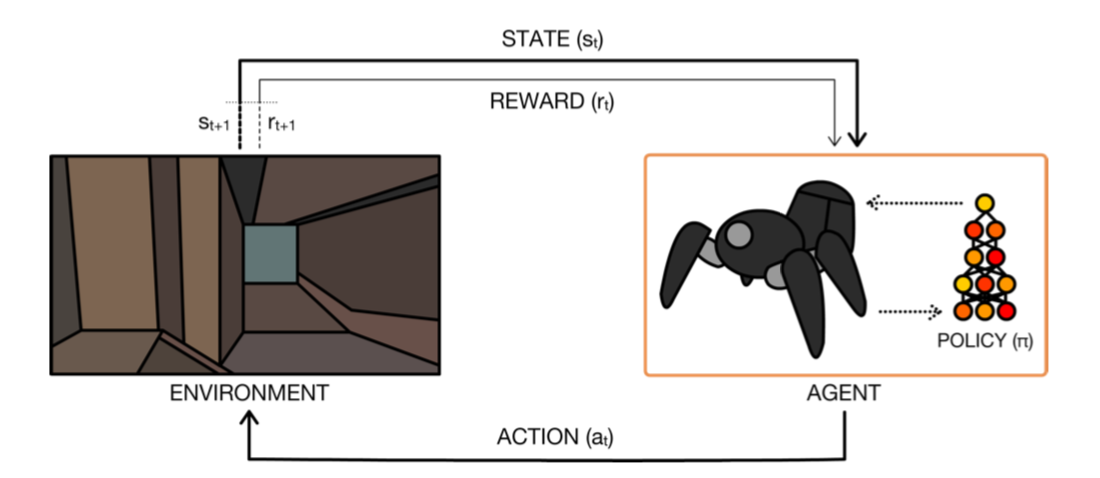
\includegraphics[width=.5\linewidth]{figures/Agent-Env.png}
  \caption{Reinforcement Learning interaction loop. The agent takes an action at a\textsubscript{t} state s\textsubscript{t}. The environment then responds with the corresponding reward r\textsubscript{t+1} and the new state s\textsubscript{t+1}, which are fed back to the agent \parencite{arulkumaran2017brief}}
  % \caption{Reinforcement Learning interaction loop. [\citetitle{sutton2018reinforcement}]}
  \label{fig:Agent_Env}
\end{center}
\end{figure}

\subsection{Environment} \label{Environment}
An Environment constitutes a world for the agent to act and learn. Our Environments could be the whole surrounding 3D space or 2D images from cameras for real world task like robotic arm, or it could represent an entire virtual world or games from an emulator like OpenAI Gym ~\parencite{brockman2016openai}.


\subsection{Markov Decision Process}
Formally, RL can be described as a Markov decision process (MDP), which consists of:

\begin{itemize}
  \item A set of states \(S\), plus a distribution of starting states \(p(s0)\).
  \item A set of actions \(A\).
  \item Transition dynamics $ \mathcal{T}\left(\mathbf{s}_{t+1} | \mathbf{s}_{t}, \mathbf{a}_{t}\right) $ that map a state-action pair at time \(t\) onto a distribution of states at time \(t+1\).
  \item An immediate $ \mathcal{R}\left(\mathbf{s}_{t}, \mathbf{a}_{t}, \mathbf{s}_{t+1}\right) $ reward function.
  \item A discount factor \(\gamma \in(0,1)\), where lower values place more emphasis on immediate rewards.
\end{itemize}

\subsection{Rewards and Return}

The reward function \(R\) is critically important in reinforcement learning. It depends on the current state of the world, the action just taken, and the next state of the world:

\begin{center}
\begin{equation}
r_{t}=R\left(s_{t}, a_{t}, s_{t+1}\right)
\end{equation}
\end{center}

The goal of the agent is to maximize some notion of cumulative reward over a trajectory.

There are two kinds of return, \textbf{the finite-horizon undiscounted return}, which is just the sum of rewards obtained in a fixed window of steps:

\begin{center}
\begin{equation} \label{eq:1}
R(\tau)=\sum_{t=0}^{T} r_{t}
\end{equation}
\end{center}

Another kind of return is \textbf{the infinite-horizon discounted return}, which is the sum of all rewards ever obtained by the agent, but \textit{discounted} by how far off in the future they’re obtained. This formulation of reward includes a discount factor \(\gamma \in(0,1)\):

\begin{center}
\begin{equation} \label{eq:2}
R(\tau)=\sum_{t=0}^{\infty} \gamma^{t} r_{t}
\end{equation}
\end{center}

The use of a discount factor is crutial as \textbf{mathematically} an infinite-horizon sum of rewards may not converge to a finite value, and is hard to deal with in equations. But with a discount factor and under reasonable conditions, the infinite sum converges.


\subsection{Value Functions}
\subsection{Policy Gradient}
\subsection{Q-Learning}
\subsection{Reinforcement learning methods}
    \subsubsection{Model-free}
    \subsubsection{Model-based}
\subsection{Limitations of RL in practice}




\section{Deep Reinforcement Learning}

\subsection{Overview}
\subsection{Deep Q Network}
\subsection{Deep Deterministic Policy Gradient}
\subsection{Proximal Policy Optimization}
\subsection{Asynchronous Advanced Actor Critic (\textbf{A3C})}

% \section{Literature Review}

\section{Challenges in Reinforcement Learning}